%Preamble
\documentclass[11pt,a4paper,twocolumn]{article}
\brokenpenalty=10000 
\hyphenpenalty=10000 
\usepackage[spanish]{babel}
\usepackage[utf8]{inputenc}
\usepackage{times}
\usepackage[T1]{fontenc}
\usepackage{tabularx} % extra features for tabular environment
\usepackage{amsmath}  % improve math presentation
\usepackage{graphicx} % takes care of graphic including machinery
\usepackage{geometry} % decreases margins
\usepackage{cite} % takes care of citations
\usepackage[final]{hyperref} % adds hyper links inside the generated pdf file
\usepackage{booktabs}
\usepackage{subcaption}
\usepackage{fancyhdr}
\usepackage{authblk}
\usepackage{parskip}
\usepackage{amssymb, amsmath} % Paquetes matemáticos de la American Mathematical Society
\usepackage{float}
\usepackage{multirow}
\usepackage[all]{xy}
\usepackage{tikz}
\usetikzlibrary{matrix}
\usetikzlibrary{calc}
\usetikzlibrary{fit}
%\usepackage{showframe}

\geometry{
    papersize = {216mm, 279mm},
    width = 20cm,
    height = 25cm,
    headsep = 5mm,
    head = 2.8cm,
    marginpar = 2mm,
    includeall,
}

\fancyhf{}
\renewcommand{\headrulewidth}{0pt}
\fancyhead[LO,LE]{
    \begin{minipage}{3cm}
        
\includegraphics[width=0.7\textwidth]{Escudo.jpg}
    \end{minipage}
}
\fancyhead[RO,RE]{
    \textsf{
        Transformada de Fourier aplicado a una función Diente de Sierra no periódica\\
        Teoría de telecomunicaciones I, Grupo A12\\
        \date{\today}   
    }
}
\fancyfoot[C]{\thepage}

\pagestyle{fancy}

\hypersetup{
	colorlinks=true,       % false: boxed links; true: colored links
	linkcolor=black,        % color of internal links
	citecolor=black,        % color of links to bibliography
	filecolor=magenta,     % color of file links
	urlcolor=blue         
}
\spanishdecimal{.}

%++++++++++++++++++++++++++++++++++++++++
%Content
\usepackage[small,compact]{titlesec}
\titleformat{\subsubsection}[runin]
            {\normalfont\it}
            {\thesubsubsection}{0.5em}{}[:]

\renewcommand*{\Authsep}{ y }
\renewcommand*{\Authand}{ y }
\renewcommand*{\Authands}{, }
\renewcommand*{\Affilfont}{\normalsize}
%\renewcommand*{\Authfont}{\bfseries}    % make author names boldface    
\setlength{\affilsep}{0.5em}   % set the space between author and affiliation

\title{
    \fontsize{26}{26}\selectfont 
    \textbf{Transformada de Fourier}}

\author[1]{Jefry Nicolás Chicaiza}
\author[2]{Jose Nicolás Zambrano}
\affil[1]{jefryn@unicauca.edu.co}
\affil[2]{jnzambranob@unicauca.edu.co}
\date{}

\begin{document}
\maketitle
\thispagestyle{fancy}
\section{Introducción}
    En el siguiente documento se desarrollará el informe del Trabajo 2 de la asignatura 
    Teoría de las telecomunicaciones 1. El trabajo presenta inicialmente el desarrollo 
    analítico de la Transformada de Fourier a la señal planteada, la cual es del tipo 
    "diente de sierra"  trasladado en el tiempo y no periódica.
    
    Iniciar con el desarrollo analítico es necesario debido a que para alcanzar los 
    resultados esperados en la simulación, se requiere conocer de antemano la función que 
    representa dicha Transformada de la señal, esto permitirá realizar una comparación
    para llegar a confirmar que se hizo una correcta adecuación del algoritmo realizado en MATLAB.
    
    
    

    Posteriormente se abordaran las hipótesis planteadas en el documento guiá del trabajo 
    y se buscará llegar a conclusiones y síntesis a partir de los datos obtenidos en la 
    simulación de los diferentes escenarios.
    
    Los teoremas e hipótesis nos dicen que la serie de Fourier de cualquier señal periódica de potencia 
    finita la podemos obtener por medio de una suma infinita de funciones sinusoidales. La serie de 
    Fourier de una señal pueden expresarse de dos maneras, una representada por serie trigonométrica y 
    otra con representación de serie compleja. 
    
    En este documento unicamente se realiza los cálculos de la serie de Fourier para la señal propuesta 
    con la representación trigonométrica, que observamos a continuación:

    \begin{equation}
        x(t)=a_{0}+\sum_{n=1}^{\infty} a_{n}cos(2\pi nf_{0}t)+b_{n}sin(2\pi f_{0}t)
        \label{equation1}
    \end{equation}
    
    Donde los términos $a_{0}$, $a_{n}$ y $b_{n}$ son los coeficientes de la serie de Fourier, de los cuales
    es necesario realizar cálculos para encontrar sus valores y lograr representar la serie de la señal dada.
   
    El desarrollo de este documento esta constituido por una sesión que brinda información 
    de como se obtuvo las diferentes expresiones y el plan de pruebas, que hacen posible la 
    implementación de variados escenarios en la simulación.
   
\section{Metodología}
    La metodología empleada para el desarrollo de la serie de Fourier a la señal planteada se 
    logro mediante la aplicación de los teoremas e hipótesis, en el apartado anterior se menciono 
    la necesidad de calcular los valores de ciertos términos para logra obtener la representación 
    matemática de la serie de Fourier de la señal planteada. 
    
    En primer lugar es importante conocer el comportamiento que nos describe los términos, el primer 
    termino de la serie, $a_{0}$, no está asociado con una frecuencia y es una constante, además es 
    conocido como el nivel DC de la señal, representa el cambio de la señal sobre un nivel arbitrario 
    de referencia. Este termino lo podemos calcular de la siguiente manera:

    \begin{equation}
        a_{0}=\frac{1}{T} \int_{T}^{} x(t)dt
        \label{equation2}
    \end{equation}
    
    De la expresión anterior podemos deducir que el termino DC representa el área bajo la curva de la 
    señal \cite{diapositivas}, que hasta el momento no conocemos la función que la representa, por tanto es necesario obtener 
    la función a partir de su gráfica. En la figura \ref{funcionAsiganda} observamos la señal asignada.

    \begin{figure}[H]
        \centering
        \selectlanguage{english}
        \begin{tikzpicture}
	        \draw[dashed, gray!20](-1,0) grid (4,3.5);
		    \draw[line width = 0.5mm, ->](-1.5,0)--(4.5, 0) node[right]{$t$};
		    \draw[line width = 0.5mm, ->](0,-0.5)--(0,4) node[above]{$x(t)$};
		    \draw[black, line width = 0.3mm](-0.5,0)--(3.5,3) node[right]{$x(t) = \dfrac{1}{4}t +\dfrac{1}{8}$};
		    \draw[black, line width = 0.3mm](3.5,0)--(3.5,3) node[right]{};
            \draw[dashed, line width = 0.2mm](0,3)--(3.5,3) node[right]{};
		    \foreach \x in {-0.5,3.5}
		    \draw (\x, 1mm)--(\x, -1mm) node [below]{\scriptsize $\x$};
		    \foreach \y in {3}		
		    \draw (1mm, \y)--(-1mm, \y) node [left]{$1$};
        \end{tikzpicture}
        \selectlanguage{spanish}
        \caption{Gráfica de la señal tipo "diente de sierra" no periódica.}
        \label{funcionAsiganda}
    \end{figure}

    En \cite{Sawtooth} se menciona que durante el intervalo en el que se presenta la señal, la función que 
    responde a una onda diente de sierra se da de la siguiente manera:
    
    \begin{equation*}
        x(t)=\frac{A}{T} t
    \end{equation*}

    Por lo que la función a la que responde la señal que se plantea debe ser del mismo modo, la expresión 
    de la señal es la siguiente:

    \begin{equation}
        x(t)=\frac{1}{4} t+\frac{1}{8}
        \label{equation3}
    \end{equation}

    Ahora que conocemos la expresión de la señal se procederá a obtener el valor del termino $a_{0}$, con las 
    ecuaciones \ref{equation2} y \ref{equation3}:

    \begin{equation*}
        a_{0}=\frac{1}{4} \int_{-\frac{1}{2}}^{\frac{7}{2}} \frac{1}{4} t+\frac{1}{8}
    \end{equation*}
    \begin{equation}
        a_{0}=\frac{1}{2}
        \label{equation4}
    \end{equation}    

    Para el valor de los términos restantes es importante mencionar que con frecuencia las simetrías simplifican 
    a los problemas matemáticos. En el caso de la series de Fourier, se utiliza la simetría en la paridad para 
    simplificar el problema. En el caso de funciones pares el desarrollo de la serie de Fourier implica solamente 
    la necesidad de calcular $a_{0}$ y $a_{n}$, y sólo $b_{n}$ para impares \cite{parimpar}.
    
    La señal que concierne a este texto podemos deducir de su gráfica(figura \ref{figure1}) que no se comporta igual que su imagen respecto 
    al eje $y$, ni tampoco hay presencia de simetría al rotar la gráfica en 180 grados. Por tanto, se trata de una 
    función sin paridad, lo que implica la necesidad de calcular todos los términos de la serie trigonométrica de Fourier .
    
    Las siguientes expresiones corresponden al calculo de los coeficientes $a_{n}$ y $b_{n}$:

    \begin{equation}
        a_{n}=\frac{2}{T} \int_{T} x(t)cos(2\pi nf_{0}t)dt
        \label{equation5}
    \end{equation}
    \begin{equation}
        b_{n}=\frac{2}{T} \int_{T} x(t)sin(2\pi nf_{0}t)dt
        \label{equation6}
    \end{equation}

    los resultados obtenidos al realizar los cálculos para los coeficientes son los siguientes (los cálculos que 
    se presentan en este documento están simplificados, por tal motivo se integra el paso a paso en el apartado de 
    Anexos):

    \begin{itemize}
        \item Calculo $a_{n}$
            \begin{equation*}
                a_{n}=\frac{1}{8}\int_{-\frac{1}{2}}^{\frac{7}{2}} tcos(2\pi nf_0t)dt + 
                \frac{1}{16} \int_{-\frac{1}{2}}^{\frac{7}{2}} cos(2\pi nf_0t)dt
            \end{equation*}
            \begin{equation}
                a_{n}=\frac{1}{\pi n} sin\left(\frac{7\pi n}{4}\right)+\frac{1}{2\pi^2 n^2}\left(cos\left(\frac{7\pi n}{4}\right)-cos\left(\frac{\pi n}{4}\right)\right)
                \label{equation7}
            \end{equation}
        \item Calculo $b_{n}$
            \begin{equation*}
                b_{n}=\frac{1}{8}\int_{-\frac{1}{2}}^{\frac{7}{2}} tsin(2\pi nf_0t)dt + 
                \frac{1}{16} \int_{-\frac{1}{2}}^{\frac{7}{2}} sin(2\pi nf_0t)dt
            \end{equation*}
            \begin{equation}
                b_{n}=-\frac{1}{\pi n} cos\left(\frac{7\pi n}{4}\right)+\frac{1}{2\pi^2 n^2}\left(sin\left(\frac{7\pi n}{4}\right)+sin\left(\frac{\pi n}{4}\right)\right)
                \label{equation8}
            \end{equation}
    \end{itemize}
    
    Lo siguiente sera completar la serie de Fourier para obtener la representación matemática de las funciones sinusoidales 
    que construyen la señal planteada, reemplazamos las ecuaciones \ref{equation7} y \ref{equation8} en la ecuación 
    \ref{equation1}:

    %\begin{multline}
        %x(t)=\frac{1}{2}+\sum_{n=1}^{\infty} \left[\frac{1}{\pi n} sin\left(\frac{7\pi n}{4}\right)+\frac{1}{2\pi^2 n^2}\left(cos\left(\frac{7\pi n}{4}\right)-cos\left(\frac{\pi n}{4}\right)\right)
        %\right]cos\left(\frac{\pi nt}{2}\right)... +\left[-\frac{1}{\pi n} cos\left(\frac{7\pi n}{4}\right)+\frac{1}{2\pi^2 n^2}\left(sin\left(\frac{7\pi n}{4}\right)+sin\left(\frac{\pi n}{4}\right)\right)
        %\right]sin\left(\frac{\pi nt}{2}\right)
        %\label{equation9}
    %\end{multline}

    %Ahora que se ha obtenido la expresión que representa la serie de Fourier de la señal, se procederá a realizar 
    un análisis de la serie de Fourier a través de una simulación realizada en computadora, en ella podremos 
    visualizar como se resuelve para cientos, o incluso miles, de componentes. Podemos comprobar qué tan buena 
    es la representación reconstruyendo la señal utilizando diferentes cantidades de componentes, para esto 
    se realizaran pruebas con un Script desarrollado en MATLAB.
    
    Después de haber realizado el planteamiento de los fundamentos matemáticos requeridos para solucionar 
    el problema, se procedió a realizar la planificación del diseño practico requerido para solucionar 
    el mismo.
    
    Se pueden identificar 6 objetivos clave a desarrollar con la simulación en MATLAB:

    \begin{enumerate}
        \item Reconstrucción de la señal dada a partir de la serie de Fourier.
        \item Justificación del número de coeficientes necesarios para ua reconstrucción adecuada de la 
            señal original.
        \item Análisis del espectro de magnitud cuando el periodo T de la señal reconstruida cambia.
        \item Análisis del espectro de magnitud cuando se agrega espacio de tiempo donde $x(t)=0$ entre 
            los pulsos periódicos "diente de sierra".
        \item Análisis de la continuidad del número de coeficientes necesarios cuando el periodo de la 
            señal cambia.
        \item Análisis de la continuidad del número de coeficientes necesarios cuando se agregan ceros 
            como en el objetivo 4.
    \end{enumerate}

    Después de realizar el análisis de los requerimientos anteriores, se plantea el siguiente \underline{esquema}
    \underline{general} para el desarrollo de la simulación:
    
   \begin{center}
         \xymatrix{
            % primera fila
            *++[F-,]\txt{1. Declaración de variables y espacios \\
                vectoriales  a utilizar} \ar[d] & &
            *++[F-,]\txt{4. Criterios utilizados para justificar el \\numero de coeficientes necesarios para \\ 
                reconstruir la señal} \ar{d}
            \\
            % segunda fila
            *++[F-,]\txt{2. Calculo de los coeficientes de Fourier} \ar[d] & &
            *++[F-,]\txt{5. Graficación de señales y espectro de la \\serie de Fourier}
            \\
            % tercer fila
            *++[F-,]\txt{3. Reconstrución de la señal a partir del \\calculo de la Serie de Fourier}
            \ar`r[ruu]`[rruu][rruu] % \ar[uuur]
        }    
    \end{center}

    Para la realización del script de simulación se utilizó el paradigma de programación estructurada, ya 
    que el mismo permite agilidad en el desarrollo del código, así como también facilita el desarrollo de los 
    planteamientos matemáticos necesarios para lograr los objetivos de la simulación.
    
    Adicionalmente la programación estructurada, brinda al observador del código una perspectiva secuencial en 
    el desarrollo del algoritmo de simulación, y, por lo tanto, un orden lógico y trazable de los resultados 
    esperados en la ejecución de este.
    
    \subsection{Plan de pruebas}
    Retomando los 6 objetivos clave a desarrollar con la simulación; se plantea el siguiente plan de pruebas 
    para cadaa uno de ellos:

    %\begin{table}[H]
        %\begin{center}
            %\begin{tabular}{| m{5cm} | m{10cm} |}
                %\hline
                %\textbf{Objetivo Clave} & \textbf{Pruebas y Criterio de Satisfacción} \\ \hline
                %\multirow{3}{4.5cm}{Reconstrucción de la señal} 
                    %& Se dibuja mediante la simulación la señal original y la señal reconstruida. \\ \cline{2-2} 
                    %& Se observan similitudes y diferencias. \\ \cline{2-2}
                    %& Se concluye si las señales son gráficamente similares o diferentes. \\ \hline
                %\multirow{4}{4.5cm}{Justificación del número de Coeficientes}
                    %& Se calcula la igualdad de Parseval. \\ \cline{2-2} 
                    %& Se observa el fenómeno de Gibbs en la vecindad delas desigualdades de la señal. \\ \cline{2-2}
                    %& Se analizan los valores obtenidos con 5 diferentes números de armónicos. \\ \cline{2-2}
                    %& Se concluye el valor de armónicos necesarios para tener una reconstrucción 
                    %aceptable de la señal. \\ \hline
                %\multirow{3}{4.5cm}{Análisis del espectro de magnitud cuando el periodo $T$ cambia}
                    %& Se dibuja y se analiza el espectro de magnitud con periodo $T=4$ y $N=100$. \\ \cline{2-2}
                    %& Se dibuja y se analiza el espectro de magnitud con el mismo $N$ y 3 valores diferentes 
                    %de periodo $T$. \\ \cline{2-2}
                    %& Se analiza las diferencias entre las gráficas. \\ \hline
                %\multirow{3}{4.5cm}{Análisis del espectro de magnitud cuando se agregan ceros}
                    %& Se dibuja y se analiza el espectro de magnitud con periodo $T_r=4$, $N=100$ y periodo de ceros $T_0=0$. \\ \cline{2-2}
                    %& Se dibuja y se analiza el espectro de magnitud con el mismo $N$, $T_r$ y 3 valores diferentes de periodo de ceros $T_0$. \\ \cline{2-2}
                    %& Se analiza las diferencias entre las gráficas. \\ \hline
                %\multirow{2}{4.5cm}{¿Número de coeficientes cambian cuando $T$ cambia?}
                    %& Se utilizan los resultados del objetivo 3 para analizar la igualdad de Parseval en cada caso. \\ \cline{2-2}
                    %& Se concluye si el valor de armónicos necesarios para tener una reconstrucción aceptable de la señal cambia o se mantiene. \\ \hline
                %\multirow{2}{4.5cm}{¿Número de coeficientes cambian cuando se agregan ceros?}
                    %& Se utilizan los resultados del objetivo 4 para analizar la igualdad de Parseval en cada caso. \\ \cline{2-2}
                    %& Se concluye si el valor de armónicos necesarios para tener una reconstrucción aceptable de la señal cambia o se mantiene. \\ \hline
            %\end{tabular}
        %\end{center}
        %\caption{Plan de pruebas.}
    %\end{table}

\section*{Análisis de Resultados}
    Para la obtención de los resultados se realizaron dos scripts en MATLAB. En el primer script se 
    realizó el calculo de los coefientes de Fourier de manera manual y se transcribieron los 
    resultados al código. En dicha simulación, los coeficientes $A_n$ cuando $n$ es mayor que 0, se 
    cancelaban. Esta primera simulación resultaba valida para reconstruir la señal original a partir de la 
    expresión de la serie de Fourier, sin embargo, evaluar los diferentes escenarios de pruebas 
    planteadas en el trabajo como agregar espacios en blanco o modificar el periodo de la señal 
    requeriría de cambios drásticos en la escritura y evaluación del código.
    
    El anterior escenario fue motivación para realizar una segunda versión del script, que permitiera 
    generalizar los escenarios planteados en el trabajo y permitiera alcanzar conclusiones completas 
    del mismo.
    
    El segundo código realiza los cálculos de los coeficientes de manera simbólica, los cuales luego son 
    evaluados en vectores numéricos aumentando así su velocidad de procesamiento. El límite 
    practico en tiempo de ejecución se encontró en un valor cercano a los 5000 armónicos. Sin 
    embargo, debido a que no es necesaria tal cantidad de cálculos, se acotó el máximo posible de 
    armónicos a 100, los cuales permiten de manera suficiente alcanzar los objetivos esperados del 
    trabajo.
    
    \textbf{Desarrollo del Objetivo Clave 1--Reconstrucción de la señal}

    \begin{figure}[H]
        \centering 
        \begin{subfigure}[h]{0.45\linewidth}
            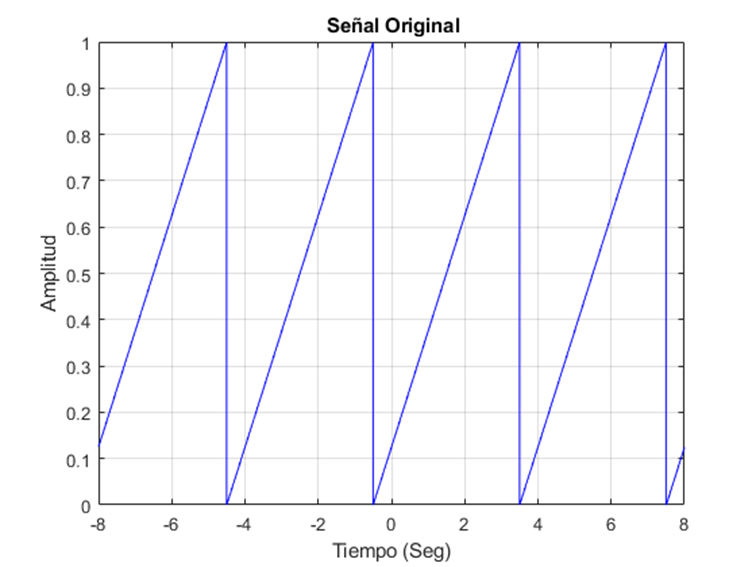
\includegraphics[width=\linewidth]{img/figure2_A.png}
            \caption{Gráfica original.}
            \label{figure2_A}
        \end{subfigure}
        \begin{subfigure}[h]{0.45\linewidth}
            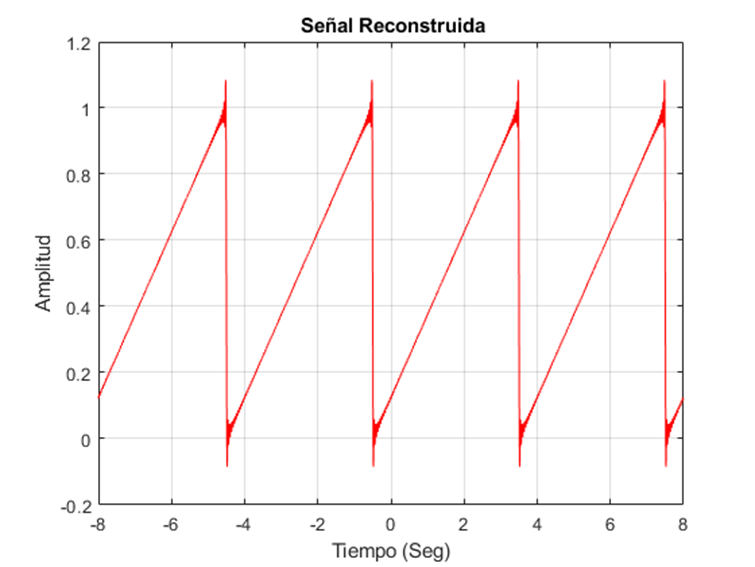
\includegraphics[width=\linewidth]{img/figure2_B.png}
            \caption{Gráfica reconstruida.}
            \label{figure2_B}
        \end{subfigure}
        \caption{Gráficas del primer script.}
        \label{figure2}
    \end{figure}

    \begin{figure}[H]
        \centering
        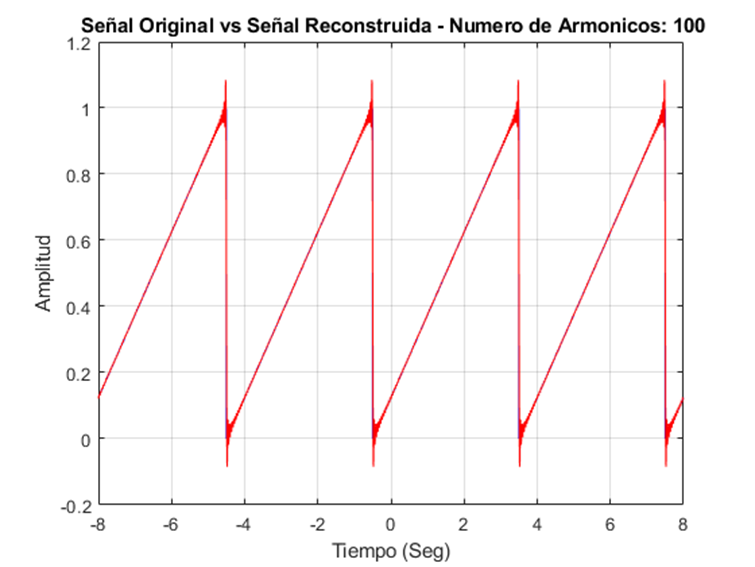
\includegraphics[width=0.5\linewidth]{img/figure3.png}
        \caption{Gráfica sobrepuestas de la señal original y reconstruida.}
        \label{figure3}
    \end{figure}

    En las figuras \ref{figure2_A}, \ref{figure2_B} y \ref{figure3} se puede observar el principal resultado visible de esta simulación: Al 
    desarrollar computacionalmente la sumatoria de la serie de Fourier se obtiene como resultado 
    una señal gráficamente muy similar a la señal original. Se observan similitudes en las regiones 
    continuas del diente de sierra o rampa. Sin embargo, como es de esperarse, las señales no son 
    completamente idénticas, ya que en los puntos de discontinuidad de la señal periódica original se 
    generan picos de amplitud explicados por el fenómeno de Gibbs. Las figuras anteriormente 
    expuestas corresponden a una simulación realizada con la sumatoria de los 100 primeros 
    armónicos. Mas adelante se abordarán escenarios de simulación con diferentes cantidades de 
    armónicos en la serie.
    
    \textbf{Desarrollo del Objetivo Clave 2--Justificación del Numero de Coeficientes}

    \begin{figure}[H]
        \centering
        \begin{subfigure}[h]{0.45\linewidth}
            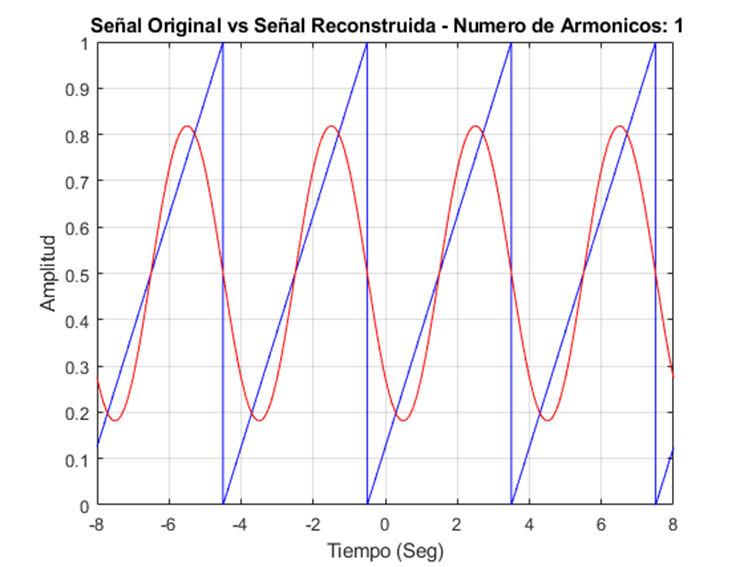
\includegraphics[width=\linewidth]{img/figure4_A.png}
            \caption{Gráfica 1 armónico.}
            \label{figure4_A}
        \end{subfigure}
        \begin{subfigure}[h]{0.45\linewidth}
            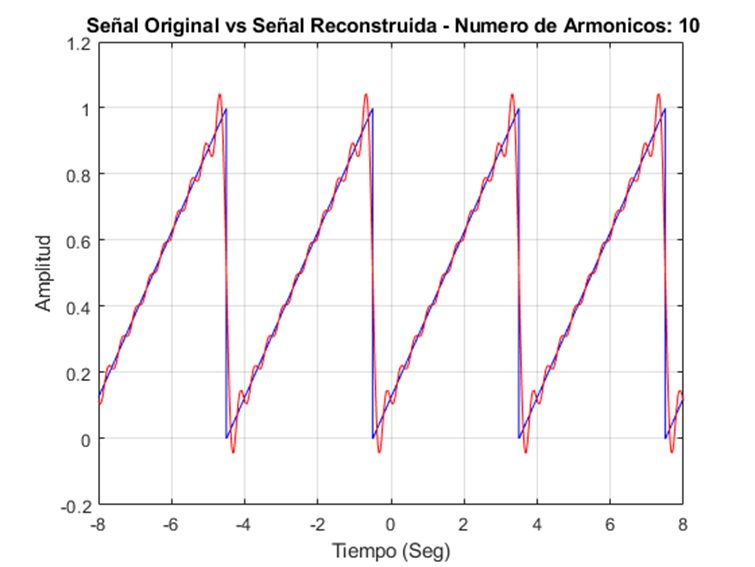
\includegraphics[width=\linewidth]{img/figure4_B.png}
            \caption{Gráfica 10 armónicos.}
            \label{figure4_B}
        \end{subfigure}
        \begin{subfigure}[h]{0.45\linewidth}
            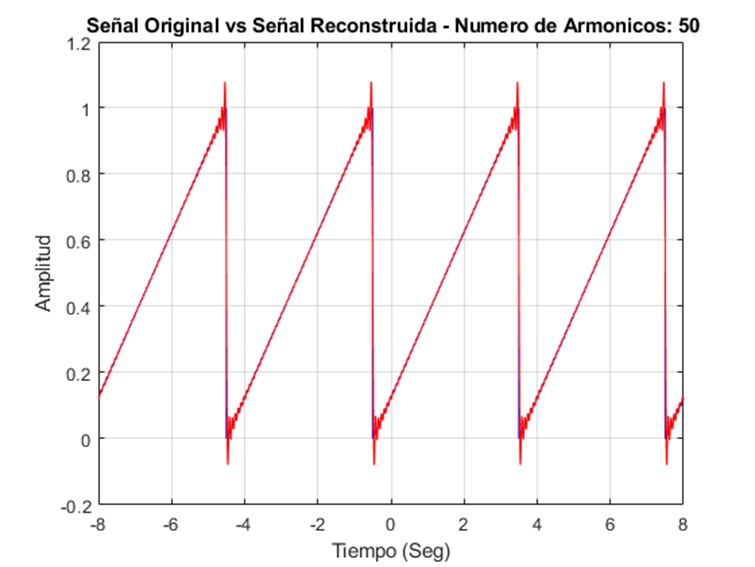
\includegraphics[width=\linewidth]{img/figure4_C.png}
            \caption{Gráfica 50 armónicos.}
            \label{figure4_C}
        \end{subfigure}
        \begin{subfigure}[h]{0.45\linewidth}
            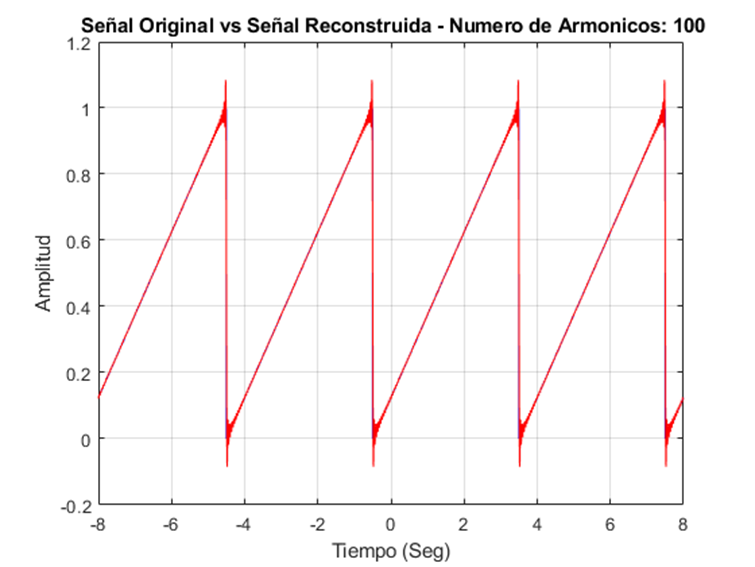
\includegraphics[width=\linewidth]{img/figure4_D.png}
            \caption{Gráfica 100 armónicos.}
            \label{figure4_D}
        \end{subfigure}
        \caption{Gráficas sobrepuestas de las señales con diferente número de armónicos.}
        \label{figure4}
    \end{figure}

    Para justificar la cantidad de coeficientes o armónicos que son necesarios para reconstruir está 
    señal de manera adecuada, se usaran dos criterios diferentes: \textbf{La igualdad de Parseval} y el 
    \textbf{fenómeno de Gibbs evaluado en el punto de la discontinuidad}.
    
    Se considerará que la cantidad de armónicos es suficiente cuando la relación entre los dos lados 
    de la igualdad de Parseval \textbf{supere el 99\% de similitud}, esto es:

    \begin{equation*}
        \frac{2}{T} \int_{0}^{T} \left|f(t)\right|^2 dt=\frac{a_{0}^2}{2} + \sum_{n=1}^{n=narm} (a_{n}^2 +b_{n}^2)
    \end{equation*}

    Por lo tanto, para encontrar el ratio de similitud proponemos la siguiente expresión:

    \begin{equation*}
        100 \frac{\frac{2}{T} \int_{0}^{T} \left|f(t)\right|^2 dt}{\frac{a_{0}^2}{2} +\sum_{n=1}^{n=narm}(a_{n}^2 +b_{n}^2)} > 99
    \end{equation*}

    Evaluando en la simulación encontramos que en el armónico $narm=15$, el ratio de 
    similitud supera el 99\% ubicándose en 99.0198\%. Esta es la señal reconstruida para ese 
    número de armónicos:
    
    \begin{figure}
       \centering 
       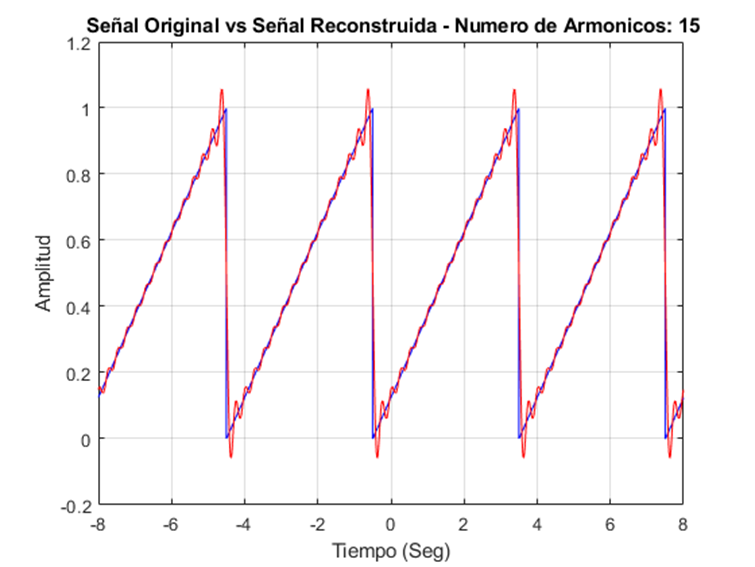
\includegraphics[width=0.5\linewidth]{img/figure5.png}
       \caption{Gráficas sobrepuestas de las señales para 15 armónicos.}
       \label{figure5}
    \end{figure}

    Como segundo criterio de confirmación de la cantidad de armónicos necesarios para la 
    reconstrucción de la señal, evaluamos la vecindad de la discontinuidad en $t=3.5$ para 
    confirmar que el valor de la señal reconstruida en la discontinuidad es igual a el valor 
    medio de la suma de los limites por la izquierda y por la derecha en la señal original, es 
    decir: 

    \begin{equation*}
       Sf(t_0) \cong \frac{f(t_0^+)+f(t_0^-)}{2}
    \end{equation*}

    donde $t_0=3.5$ que es el valor de la discontinuidad. Al evaluar en la simulación 
    confirmamos que:
    
     $Sf(t_0)=\frac{f(t_0^+)+f(t_0^-)}{2}=0.5000$ por lo que se confirma que el fenómeno de Gibbs 
     en la desigualdad converge a su valor medio. Por lo tanto, verificamos que 15 armónicos 
     son suficientes para tener una reconstrucción aceptable de la señal. 
     
     \textbf{Desarrollo del Objetivo Clave 3 -- Análisis del espectro de magnitud cuando el periodo $T$ cambia}
     
     
     Para desarrollar este objetivo clave se realizaron 4 escenarios diferentes de simulación variando la 
     duración del diente de sierra, es decir, su periodo. Se realiza las simulaciones con un número 
     de 100 armónicos; esto se hace para poder apreciar mejor el espectro de magnitud 
     discreto con los 100 valores obtenidos.

    \begin{figure}[H]
        \centering
        \begin{subfigure}[h]{0.45\linewidth}
            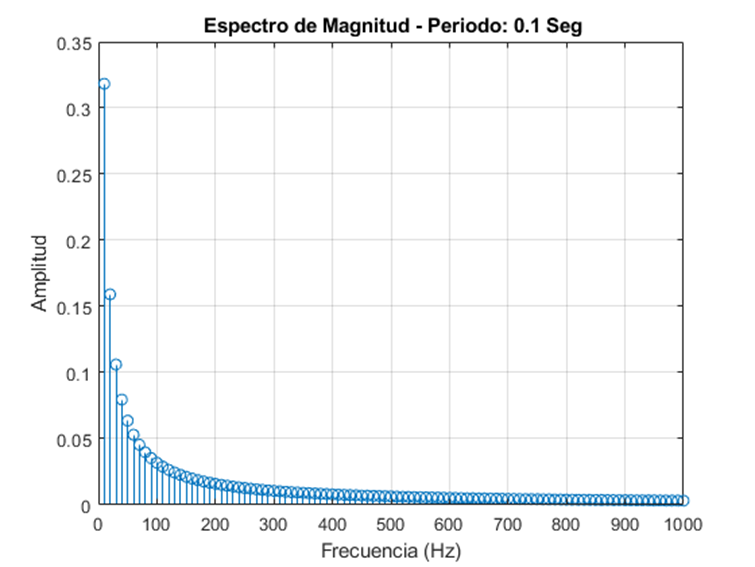
\includegraphics[width=\linewidth]{img/figure6_A.png}
            \caption{Gráfica 0.1 segundos.}
            \label{figure6_A}
        \end{subfigure}
        \begin{subfigure}[h]{0.45\linewidth}
            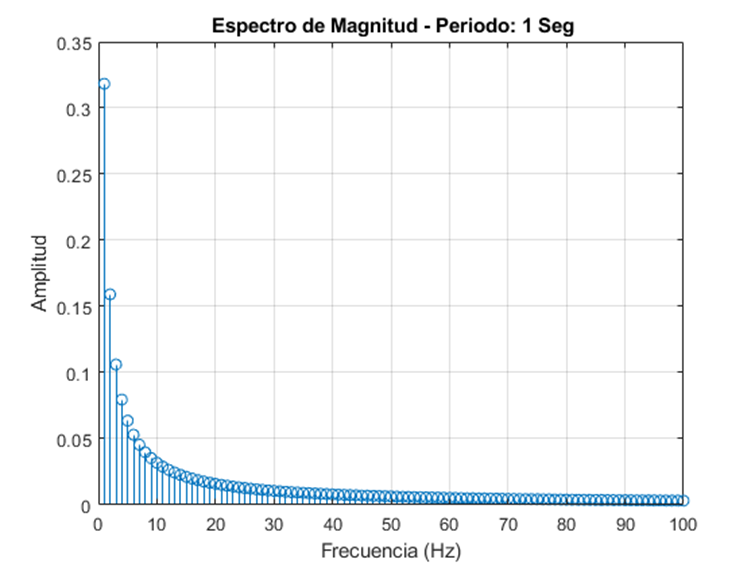
\includegraphics[width=\linewidth]{img/figure6_B.png}
            \caption{Gráfica 1 segundo.}
            \label{figure6_B}
        \end{subfigure}
        \begin{subfigure}[h]{0.45\linewidth}
            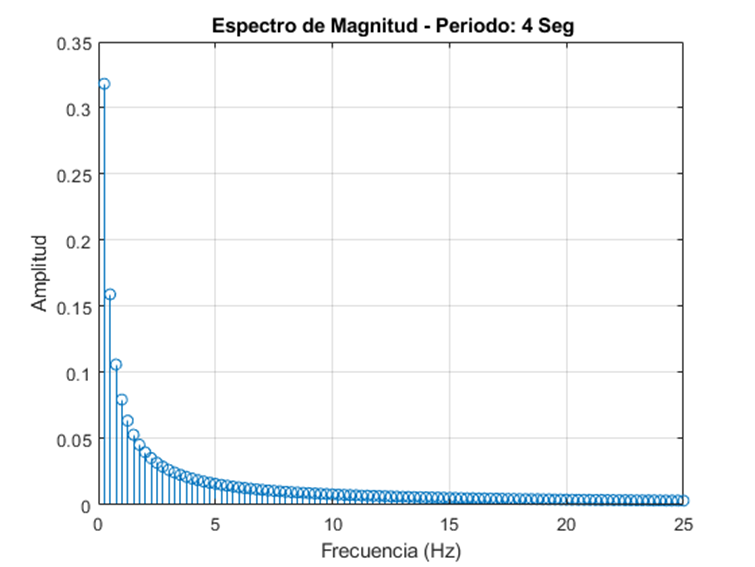
\includegraphics[width=\linewidth]{img/figure6_C.png}
            \caption{Gráfica 4 segundos.}
            \label{figure6_C}
        \end{subfigure}
        \begin{subfigure}[h]{0.45\linewidth}
            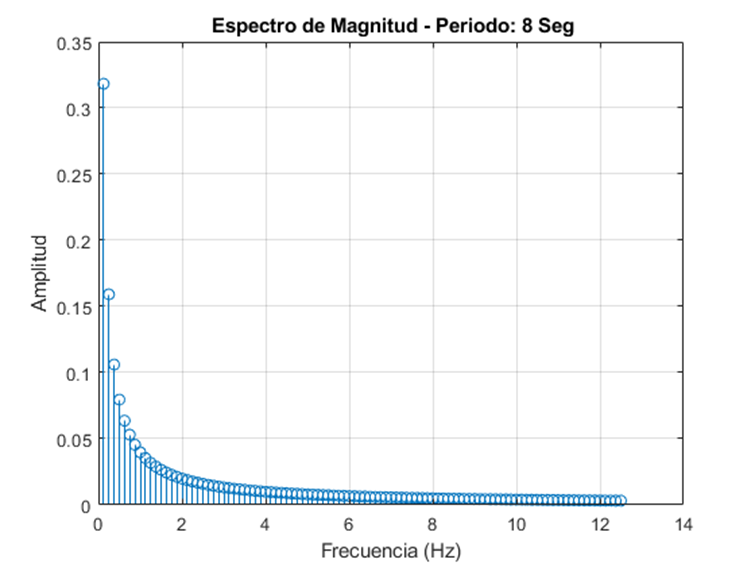
\includegraphics[width=\linewidth]{img/figure6_D.png}
            \caption{Gráfica 8 segundos.}
            \label{figure6_D}
        \end{subfigure}
        \caption{Gráficas del espectro de magnitud en 4 valores de $T$ diferentes.}
        \label{figure6}
    \end{figure}

    se puede apreciar que las magnitudes de cada armónico se mantienen iguales en todos 
    los periodos simulados. Esto indica que el \textbf{cambio en el periodo de la señal no afecta a las 
    magnitudes} debido a que la \textbf{forma de la señal periódica permanece igual y el periodo es 
    compensado por el cambio de la pendiente de la rampa}, por lo cual las integrales que 
    definen a los coeficientes permanecen iguales ya que sus periodos se normalizan. Para el 
    periodo afecta directamente a la frecuencia.
    
    Se puede concluir que un cambio en el periodo de la señal únicamente cambia el valor de 
    frecuencia normalizada al que pertenece cada armónico. Para periodos mas pequeños, se 
    tiene que la frecuencia aumente, y para periodos grandes la frecuencia disminuye tal cual 
    la definición formal de frecuencia:
    
    \begin{equation}
        f=\frac{1}{T}
    \end{equation}

     \textbf{Desarrollo del Objetivo Clave 4 -- Análisis del espectro de magnitud cuando se agregan ceros}

     En este escenario se simulan ceros añadidos al terminar cada diente de sierra; el periodo del 
     diente se mantiene constante en 4 segundos, y se varia la longitud de los ceros en 4 escenarios: sin 
     ceros, 4 segundos, 8 segundos y 100 segundos de ceros. El periodo se esta \textbf{nueva señal resultante}
     está definido por: $T=\frac{1}{T_0+T_r}$ donde $T_0$ es el periodo de duración de los ceros y $T_r$ es el periodo 
     del pulso diente de sierra. Este cambio en el periodo completo de la señal afecta directamente el 
     calculo de los coeficientes debido al cambio que existe en la frecuencia fundamental dentro de las 
     integrales. Para estos casos, los coeficientes $A_n$ ya no se cancelan y se forman otro tipo de 
     coeficientes basados en la función seno cardinal.

    \begin{figure}[H]
        \centering
        \begin{subfigure}[h]{0.45\linewidth}
            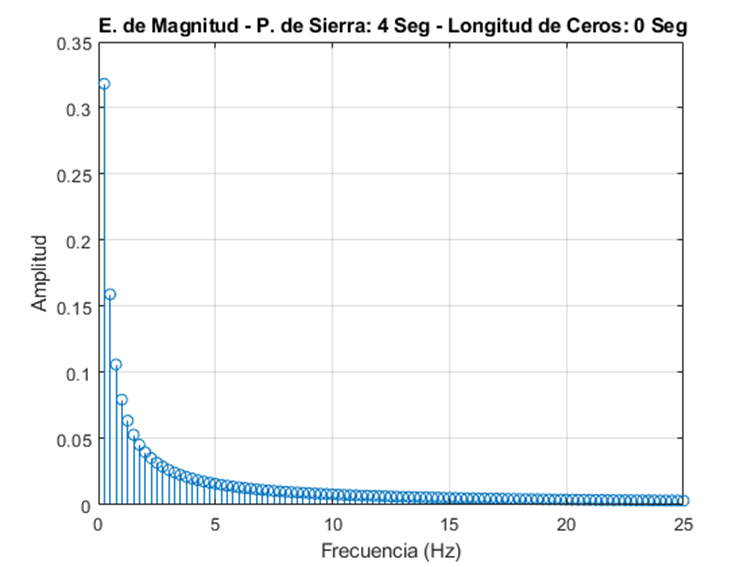
\includegraphics[width=\linewidth]{img/figure7_A.png}
            \caption{Gráfica 0 segundos.}
            \label{figure7_A}
        \end{subfigure}
        \begin{subfigure}[h]{0.45\linewidth}
            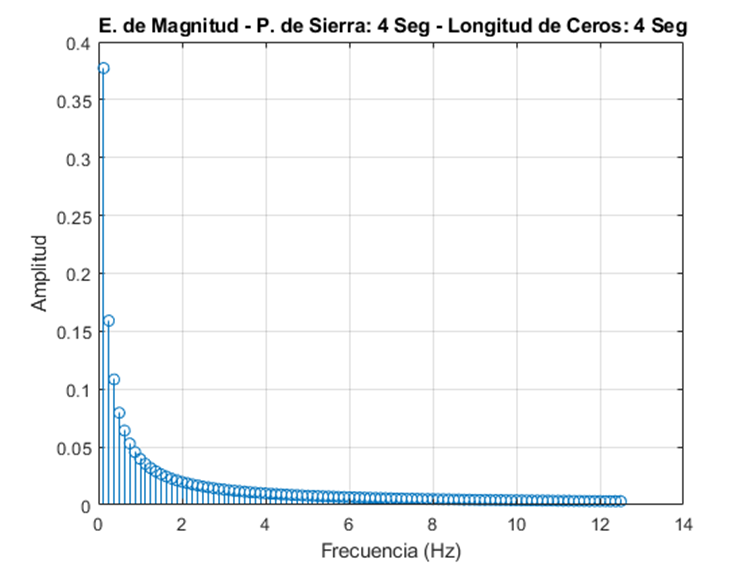
\includegraphics[width=\linewidth]{img/figure7_B.png}
            \caption{Gráfica 4 segundos.}
            \label{figure7_B}
        \end{subfigure}
        \begin{subfigure}[h]{0.45\linewidth}
            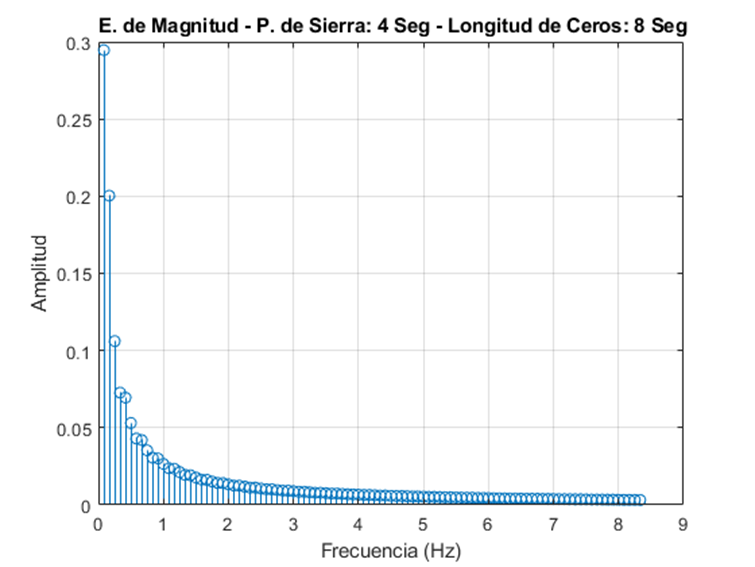
\includegraphics[width=\linewidth]{img/figure7_C.png}
            \caption{Gráfica 8 segundos.}
            \label{figure7_C}
        \end{subfigure}
        \begin{subfigure}[h]{0.45\linewidth}
            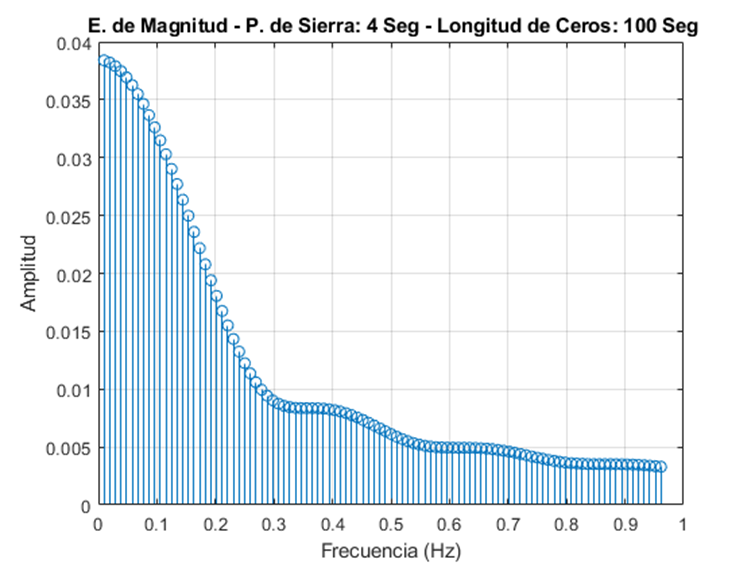
\includegraphics[width=\linewidth]{img/figure7_D.png}
            \caption{Gráfica 100 segundos.}
            \label{figure7_D}
        \end{subfigure}
        \caption{Gráficas del espectro de magnitud en 4 valores de $T$ diferentes.}
        \label{figure7}
    \end{figure}

    Se puede evidenciar que para este caso si existen cambios en las componentes del 
    espectro de magnitud. Hay tres cambios principales:

    \begin{enumerate}
        \item Cambio en la amplitud de las magnitudes de los armónicos, los cuales tienden a 
            disminuir cuando se aumenta la longitud de los ceros. Esto nos indica que entre 
            mas se aumenten los ceros, la magnitud y por lo tanto la energía de la señal tiende 
            a cero.
        \item Cambio en la frecuencia normalizada de cada armónico debido al cambio de la 
            frecuencia de la nueva señal resultante.
        \item Cambio en la diferencia de magnitud entre cada armónico la cual se presenta 
            porque todos los armónicos sin excepción tienden a aproximarse a cero.
    \end{enumerate}

    En la ultima gráfica puede apreciarse que la envolvente del espectro de magnitud tiene la 
    forma de un seno cardinal rectificado, pero sin cruces por cero, esto debido al cambio en 
    la composición de los coeficientes antes mencionada.

    \textbf{Desarrollo del Objetivo Clave 5 -- ¿El número de coeficientes requeridos cambian cuando $T$ cambia?}
    
    Los valores que se toman para este escenario son $T=(0.1,1,4,8,100)$, es decir, los mismos 
    periodos que para el Objetivo 3 sin ceros añadidos; se adiciona el valor de 100 para llevar el 
    periodo a un valor mucho más grande que el valor del periodo original de la señal. En esta 
    ocasión se limita a simular y comparar los resultados de la identidad de Parseval para cada uno de 
    los periodos a evaluar y a observar el fenómeno de Gibbs en las discontinuidades, como se hizo en 
    el Objetivo 2.

    %\begin{table}[H]
        %\begin{center}
            %\begin{tabular}{| m{2.5cm} | m{2.5cm} | m{2.5cm} | m{2.5cm} | m{2.5cm} |}
                %\hline
                %\textbf{Número de Armónicos} & \textbf{Periodo} & \textbf{Valor de la Relación de Parseval} & \textbf{Valor de la Serie en la discontinuidad} & \textbf{Valor medio en la discontinuidad}  \hline
                %15 & 0.1 & 99.0198 & 0.5 & 0.5 \\ \hline
                %15 & 1 & 99.0198 & 0.5 & 0.5 \\ \hline
                %15 & 4 & 99.0198 & 0.5 & 0.5 \\ \hline
                %15 & 8 & 99.0198 & 0.4850 & 0.5 \\ \hline
                %15 & 100 & 99.0198 & 0.5 & 0.5 \\ \hline
            %\end{tabular}
        %\end{center}
    %\end{table}

    De los valores en la tabla se puede concluir que el cambio en el periodo del diente de 
    sierra no afecta el número de armónicos requeridos como mínimo para reconstruir la 
    señal. Esto ocurre debido a que las funciones periódicas que componen a los coeficientes 
    se ajustan proporcionalmente al ancho del pulso, modificando de forma proporcional su 
    frecuencia fundamental.
    
    Para el caso del valor de la serie en la discontinuidad para el periodo $T=8$, este desfase 
    ocurre porque la simulación computarizada no tiene valores infinitos para definir el vector 
    de tiempo y el vector de la serie de Fourier. Todos los valores son discretos, por lo que hay 
    escenarios en los cuales el tiempo $t$ no esta definido para el valor exacto donde se 
    presenta la discontinuidad. Esto hace que se presente un error de cuantificación el cual se 
    evade parcialmente en la simulación encontrando el valor más cercano a la discontinuidad 
    y tomando ese valor.
    
    \textbf{Desarrollo del Objetivo Clave 6 -- ¿El número de coeficientes requeridos cambian cuando se agregan ceros}
    
    Tomando como referencia los mismos valores del Objetivo 4; se simulan los mismos 
    escenarios: $T_0=(0,4,8,100,1000)$. Se agrega el valor de 1000 con el objetivo de evaluar si la 
    forma de la señal reconstruida mantiene su integridad. El periodo de la rampa se mantiene 
    constante en 4 segundos.

    %\begin{table}[H]
        %\begin{center}
            %\begin{tabular}{| m{2.5cm} | m{2.5cm} | m{2.5cm} | m{2.5cm} | m{2.5cm} |}
                %\hline
                %\textbf{Número de Armónicos} & \textbf{Periodo de duración de los ceros} & \textbf{Valor de la Relación de Parseval} & \textbf{Valor de la Serie en la discontinuidad} & \textbf{Valor medio en la discontinuidad} \\ \hline
                %15 & 0 & 99.0198 & 0.5 & 0.5 \\ \hline
                %15 & 4 & 98.0391 & 0.5087 & 0.5 \\ \hline
                %15 & 8 & 97.0611 & 0.5095 & 0.5 \\ \hline
                %15 & 100 & 70.4557 & 0.5015 & 0.5 \\ \hline
                %15 & 1000 & 9.2372 & 0.0616 & 0.5 \\ \hline
            %\end{tabular}
        %\end{center}
    %\end{table}

    Es evidente que al igual que en el objetivo 4, el agregar ceros a la función original modifica 
    de manera importante a la señal reconstruida. Para este caso se observa que, para cada 
    escenario de simulación, es necesario aumentar el numero de armónicos si se quiere 
    continuar con el criterio de aceptación de la señal.

    \begin{figure}[H]
        \centering 
        \begin{subfigure}[h]{0.45\linewidth}
            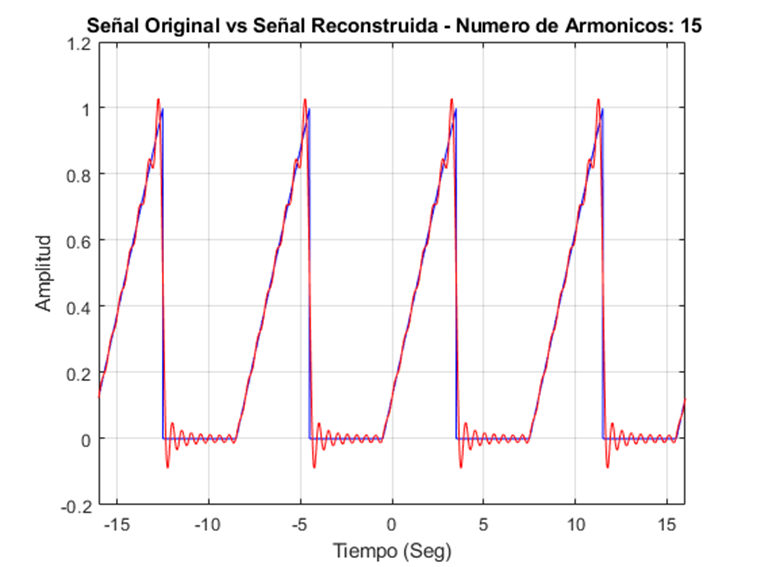
\includegraphics[width=\linewidth]{img/figure8_A.png}
            \caption{Gráfica de la señal reconstruida sobrepuesta a la original para un periodo de ceros de 4 segundos.}
            \label{figure8_A}
        \end{subfigure}
        \begin{subfigure}[h]{0.45\linewidth}
            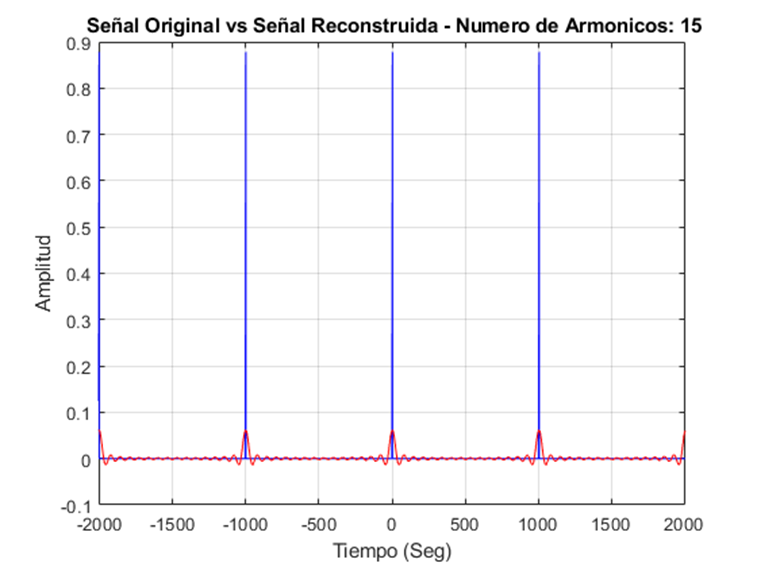
\includegraphics[width=\linewidth]{img/figure8_B.png}
            \caption{Gráfica de la señal reconstruida sobrepuesta a la original para un periodo de ceros de 1000 segundos.}
            \label{figure8_B}
        \end{subfigure}
        \label{figure8}
    \end{figure}

    Se encuentra por sustitución el número de armónicos requeridos para obtener 
    nuevamente el criterio establecido del 99 por ciento, encontrando así los siguientes 
    valores:

    %\begin{table}[H]
        %\begin{center}
            %\begin{tabular}{| m{2.5cm} | m{2.5cm} | m{2.5cm} | m{2.5cm} | m{2.5cm} |}
                %\hline
                %\textbf{Número de Armónicos} & \textbf{Periodo de duración de los ceros} & \textbf{Valor de la Relación de Parseval} & \textbf{Valor de la Serie en la discontinuidad} & \textbf{Valor medio en la discontinuidad} \\ \hline
                %15 & 0 & 99.0198 & 0.5 & 0.5 \\ \hline
                %30 & 4 & 99.0034 & 0.5266 & 0.5 \\ \hline
                %46 & 8 & 99.0192 & 0.4662 & 0.5 \\ \hline
                %395 & 100 & 99.0009 & 0.2371 & 0.5 \\ \hline
                %3815 & 1000 & 99.0002 & 0.8631 & 0.5 \\ \hline
            %\end{tabular}
        %\end{center}
    %\end{table}

    Se concluye que el número de armónicos requeridos para tener una reconstrucción 
    adecuada de la señal aumenta proporcionalmente a la duración del periodo de ceros 
    añadido.

    \begin{figure}[H]
        \centering 
        \begin{subfigure}[h]{0.45\linewidth}
            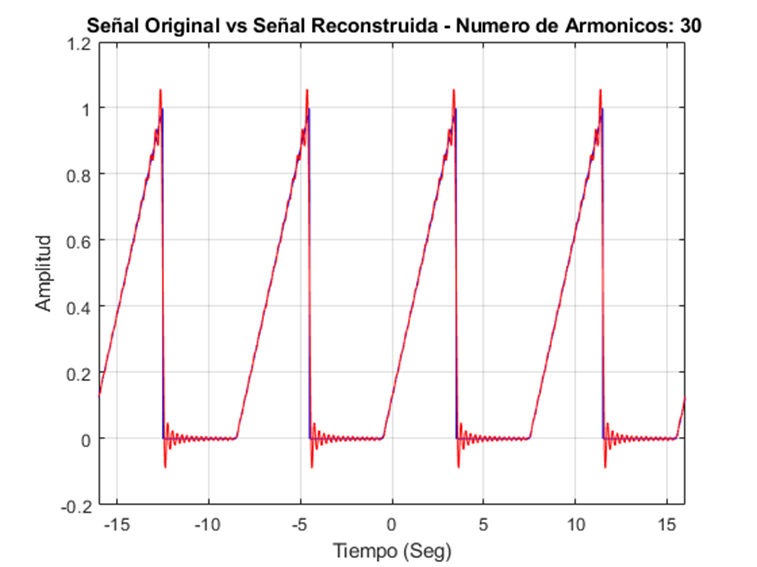
\includegraphics[width=\linewidth]{img/figure9_A.png}
            \caption{Señal de periodo de ceros 4 seg. reconstruida con los armónicos requeridos.}
            \label{figure9_A}
        \end{subfigure}
        \begin{subfigure}[h]{0.45\linewidth}
            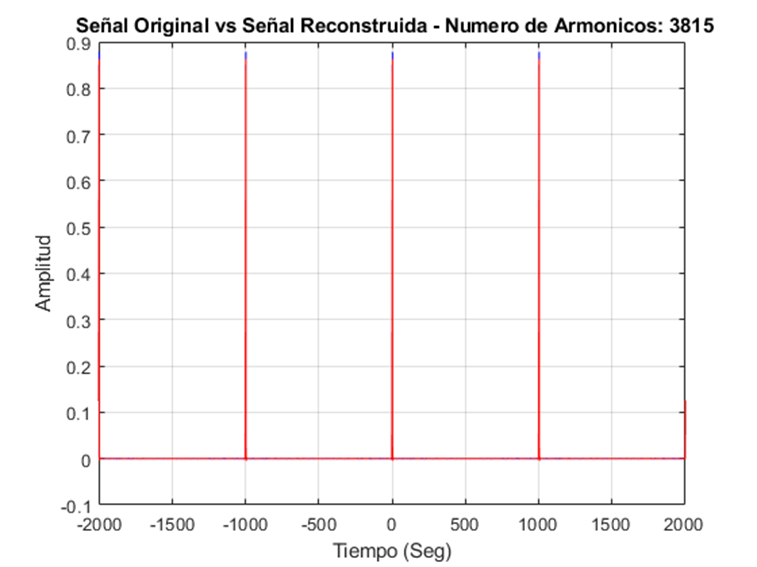
\includegraphics[width=\linewidth]{img/figure9_B.png}
            \caption{Señal de periodo de ceros 1000 seg. reconstruida con los armónicos requeridos.}
            \label{figure9_B}
        \end{subfigure}
        \label{figure9}
    \end{figure}
        
    Sin embargo, a pesar de que el criterio de la igualdad de Parseval se puede mantener, no 
    se puede decir lo mismo del criterio de Gibbs. Esto ocurre debido a que, para valores del 
    periodo de ceros muy grande, el \textbf{fenómeno de Gibbs} añade demasiada oscilación en la 
    vecindad de la discontinuidad. Una forma de solucionar esto es aumentar el tiempo de 
    muestreo en el vector del tiempo (eje de abscisas para la serie), sin embargo, el tiempo 
    computacional requerido por el número de armónicos tan grande crecería, además, 
    proporcionalmente al aumento en el valor del muestreo; Por lo que la simulación se toma 
    computacionalmente difícil.

    \begin{figure}[H]
        \centering
        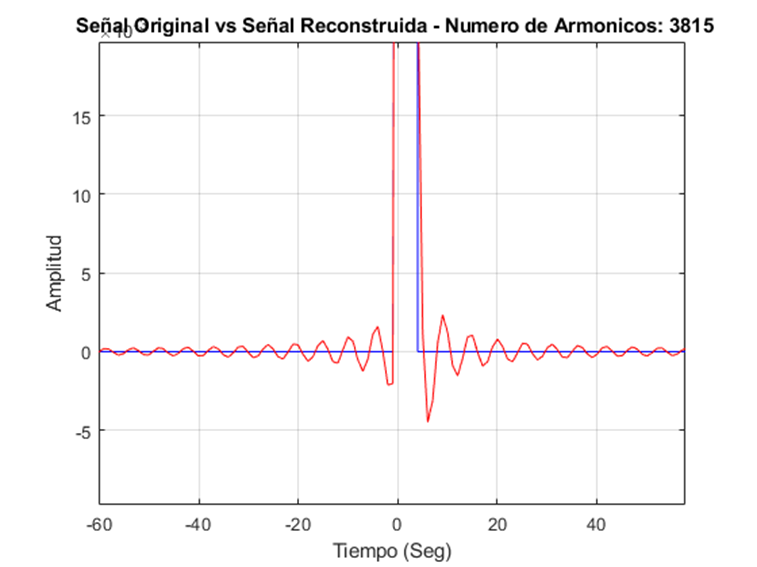
\includegraphics[width=0.5\textwidth]{img/figure10.png}
        \caption{Fenómeno de Gibbs evidenciado en la señal de periodo de ceros de 1000 segundos.}
        \label{figure10}
    \end{figure}

\section*{Conclusiones}
    
    Se concluye que una adecuada optimización del código es necesaria para la evaluación de cantidades 
    considerables de armónicos. Una inadecuada implementación del código puede llevar a hacer inviable 
    la simulación en situaciones de múltiples repeticiones. Además el uso de cálculos numéricos en vez 
    de cálculos simbólicos acelera el tiempo de ejecución del algoritmo de simulación.
    
    Un adecuado plan de pruebas es necesario antes de iniciar con la construcción de un algoritmo 
    de simulación. Esto debido a que si se inicia construyendo primero la simulación, se corre el 
    riesgo de perder trabajo debido a un inadecuado planteamiento del algoritmo.
    
    La igualdad de Parseval es una herramienta simple y adecuada para evaluar si la reconstrucción de 
    una señal a partir de la serie de Fourier es adecuada o no. Por otro lado, el criterio de Gibbs 
    presenta dificultades para su evaluación en sistemas de tiempo discreto como lo es una simulación 
    computacional. Esto debido a la incertidumbre generada en los puntos de desigualdad y al error de 
    cuantificación que se introduce debido a ello.
    
    Agregar ceros entre las repeticiones de un pulso periódico causa que el espectro de magnitud 
    se empiece a asemejar al espectro de magnitud de un tren de pulsos rectangulares. Otro aspecto a 
    considerar es el desplazamiento temporal de una función periódica no causa modificaciones a su espectro 
    magnitud. 

\begin{thebibliography}{99}
    \bibitem{diapositivas}
        M. Silva, “Capítulo II: Análisis de Fourier,” Notas Cl., pp. 3–70, 2021.
    \bibitem{Sawtooth}
        A. Engineering, M. Subject, L. Transform, and O. F. Periodic, “Snpit \& rc,” p. 11, [Online]. Available: https://www.slideshare.net/surtikaushal/laplace-periodic-function-with-graph.
    \bibitem{parimpar}
        E. Rojero, “Matemáticas Avanzadas,” Univ. Nac. Autónoma México, vol. 0.1, p. 52, 2009, [Online]. Available: https://openlibra.com/es/book/download/matematicas-avanzadas.
\end{thebibliography}
\end{document}
